\documentclass[a4paper,10pt]{report}
\usepackage[utf8]{inputenc}
\usepackage{graphicx}
\usepackage{float}
\usepackage{tikz}
\usepackage{pgfplots}

%\usepackage{geometry}
% \geometry{
% a4paper,
% total={170mm,257mm},
% left=20mm,
% top=20mm,
% }

\usepackage[margin=1in]{geometry}

% Title Page
\title{Results and Analysis}
\author{Kapil Thakkar and Reshma Kumari}


\begin{document}
\maketitle

% \chapter{Results and Analysis}

\begin{figure}[H]
\centering
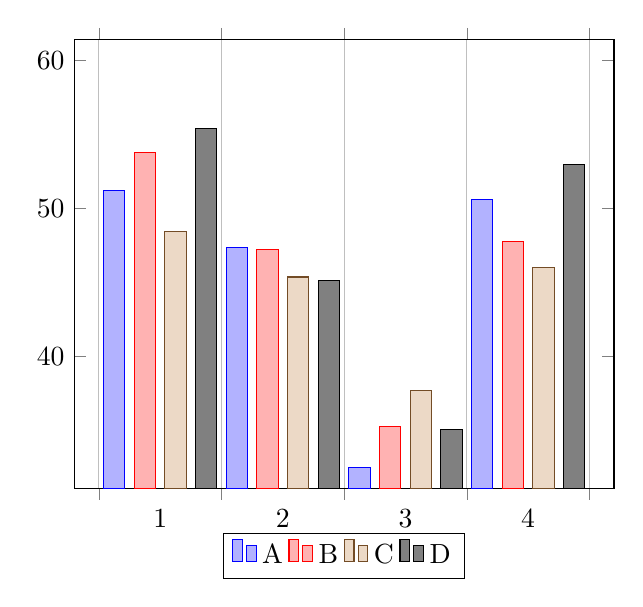
\begin{tikzpicture}
\begin{axis}[
	x tick label style={
		/pgf/number format/1000 sep=},
	enlargelimits=0.05,
	legend style={at={(0.5,-0.1)},
	anchor=north,legend columns=-1},
	ybar interval=0.7,
]

\addplot 
	coordinates {(1,51.2) (2,47.37)
		 (3,32.5) (4,50.6) (5,60)};
\addplot 
	coordinates {(1,53.78) (2,47.24)
		 (3,35.26) (4,47.74) (5,60)};
\addplot 
	coordinates {(1,48.45) (2,45.37)
		 (3,37.72) (4,46.02) (5,60)};
\addplot 
	coordinates {(1,55.4) (2,45.16)
		 (3,35.09) (4,52.98) (5,60)};	
		 
		 
\legend{A, B, C, D}
\end{axis}
\end{tikzpicture}
\caption{Anomaly Reported, (1-Retail vs Average Retail, 2-Retail vs Arrival, 3-Retail vs Wholesale, 4-Wholesale vs Arrival)}
\label{fig:comparisonMultipleWindows}
\end{figure}

Where,
\begin{itemize}
 \item A - System result when Correlation Window: 15 and Slope Based Window: 7
 \item B - System result when Correlation Window: 10 and Slope Based Window: 4
 \item C - System result when Correlation Window: 20 and Slope Based Window: 4
 \item D - System result when Correlation Window: 7 and Slope Based Window: 4
\end{itemize}


Figure \ref{fig:comparisonMultipleWindows} shows comparison of system result taking different window size for correlation and slope based anomaly detection mathod. Note that for all of these methods, default threshold value was considered, user did not provided threshold value in any. From this figure \ref{fig:comparisonMultipleWindows}, we can see that analysis where both series are inversely proportional to each other, A is performing better. Where both series are directly proportional to each other reducing window size for correlation method does help as we can see by comparing A, B and D.

\end{document}          
